\documentclass{beamer}
\mode<presentation>{
  \usetheme{Boadilla}
  \usefonttheme[onlylarge]{structurebold}
  \usefonttheme[stillsansseriflarge]{serif}
  \setbeamerfont*{frametitle}{size=\normalsize,series=\bfseries}
  % \setbeamertemplate{navigation symbols}{}
  \setbeamercovered{transparent}
}
\usepackage[english]{babel}
\usepackage[latin1]{inputenc}
\usepackage{times}
\usepackage[T1]{fontenc}
\usepackage{amsmath}
\usepackage{amssymb}
\usepackage{esint}
\usepackage{hyperref}
\usepackage{tikz}
\usepackage{xkeyval}
\usepackage{xargs}
\usepackage{verbatim}
\usepackage{listings}
\usepackage{multimedia}
\usepackage{bm}
\usepackage{siunitx}
\usetikzlibrary{
  arrows,
  calc,
  decorations.pathmorphing,
  decorations.pathreplacing,
  decorations.markings,
  fadings,
  positioning,
  shapes
}

\mode<handout>{
  \usepackage{pgfpages}
  \pgfpagesuselayout{4 on 1}[a4paper,landscape,border shrink=5mm]
  \setbeamercolor{background canvas}{bg=black!10}
}

\newcommand\pgfmathsinandcos[3]{%
  \pgfmathsetmacro#1{sin(#3)}%
  \pgfmathsetmacro#2{cos(#3)}%
}
\newcommand\LongitudePlane[3][current plane]{%
  \pgfmathsinandcos\sinEl\cosEl{#2} % elevation
  \pgfmathsinandcos\sint\cost{#3} % azimuth
  \tikzset{#1/.estyle={cm={\cost,\sint*\sinEl,0,\cosEl,(0,0)}}}
}
\newcommand\LatitudePlane[3][current plane]{%
  \pgfmathsinandcos\sinEl\cosEl{#2} % elevation
  \pgfmathsinandcos\sint\cost{#3} % latitude
  \pgfmathsetmacro\yshift{\cosEl*\sint}
  \tikzset{#1/.estyle={cm={\cost,0,0,\cost*\sinEl,(0,\yshift)}}} %
}
\newcommand\DrawLongitudeCircle[2][1]{
  \LongitudePlane{\angEl}{#2}
  \tikzset{current plane/.prefix style={scale=#1}}
  % angle of "visibility"
  \pgfmathsetmacro\angVis{atan(sin(#2)*cos(\angEl)/sin(\angEl))} %
  \draw[current plane] (\angVis:1) arc (\angVis:\angVis+180:1);
  \draw[current plane,dashed] (\angVis-180:1) arc (\angVis-180:\angVis:1);
}
\newcommand\DrawLatitudeCircleArrow[2][1]{
  \LatitudePlane{\angEl}{#2}
  \tikzset{current plane/.prefix style={scale=#1}}
  \pgfmathsetmacro\sinVis{sin(#2)/cos(#2)*sin(\angEl)/cos(\angEl)}
  % angle of "visibility"
  \pgfmathsetmacro\angVis{asin(min(1,max(\sinVis,-1)))}
  \draw[current plane,decoration={markings, mark=at position 0.6 with {\arrow{<}}},postaction={decorate},line width=.6mm] (\angVis:1) arc (\angVis:-\angVis-180:1);
  \draw[current plane,dashed,line width=.6mm] (180-\angVis:1) arc (180-\angVis:\angVis:1);
}
\newcommand\DrawLatitudeCircle[2][1]{
  \LatitudePlane{\angEl}{#2}
  \tikzset{current plane/.prefix style={scale=#1}}
  \pgfmathsetmacro\sinVis{sin(#2)/cos(#2)*sin(\angEl)/cos(\angEl)}
  % angle of "visibility"
  \pgfmathsetmacro\angVis{asin(min(1,max(\sinVis,-1)))}
  \draw[current plane] (\angVis:1) arc (\angVis:-\angVis-180:1);
  \draw[current plane,dashed] (180-\angVis:1) arc (180-\angVis:\angVis:1);
}
\newcommand\coil[1]{
  {\rh * cos(\t * pi r)}, {\apart * (2 * #1 + \t) + \rv * sin(\t * pi r)}
}
\makeatletter
\define@key{DrawFromCenter}{style}[{->}]{
  \tikzset{DrawFromCenterPlane/.style={#1}}
}
\define@key{DrawFromCenter}{r}[1]{
  \def\@R{#1}
}
\define@key{DrawFromCenter}{center}[(0, 0)]{
  \def\@Center{#1}
}
\define@key{DrawFromCenter}{theta}[0]{
  \def\@Theta{#1}
}
\define@key{DrawFromCenter}{phi}[0]{
  \def\@Phi{#1}
}
\presetkeys{DrawFromCenter}{style, r, center, theta, phi}{}
\newcommand*\DrawFromCenter[1][]{
  \setkeys{DrawFromCenter}{#1}{
    \pgfmathsinandcos\sint\cost{\@Theta}
    \pgfmathsinandcos\sinp\cosp{\@Phi}
    \pgfmathsinandcos\sinA\cosA{\angEl}
    \pgfmathsetmacro\DX{\@R*\cost*\cosp}
    \pgfmathsetmacro\DY{\@R*(\cost*\sinp*\sinA+\sint*\cosA)}
    \draw[DrawFromCenterPlane] \@Center -- ++(\DX, \DY);
  }
}
\newcommand*\DrawFromCenterText[2][]{
  \setkeys{DrawFromCenter}{#1}{
    \pgfmathsinandcos\sint\cost{\@Theta}
    \pgfmathsinandcos\sinp\cosp{\@Phi}
    \pgfmathsinandcos\sinA\cosA{\angEl}
    \pgfmathsetmacro\DX{\@R*\cost*\cosp}
    \pgfmathsetmacro\DY{\@R*(\cost*\sinp*\sinA+\sint*\cosA)}
    \draw[DrawFromCenterPlane] \@Center -- ++(\DX, \DY) node {#2};
  }
}
\makeatother

% not mandatory, but I though it was better to set it blank
\setbeamertemplate{headline}{}
\def\beamer@entrycode{\vspace{-\headheight}}

\tikzstyle{snakearrow} = [decorate, decoration={pre length=0.2cm,
  post length=0.2cm, snake, amplitude=.4mm,
  segment length=2mm},thick, ->]

%% document-wide tikz options and styles

\tikzset{%
  % >=latex, % option for nice arrows
  inner sep=0pt,%
  outer sep=2pt,%
  mark coordinate/.style={inner sep=0pt,outer sep=0pt,minimum size=3pt,
    fill=black,circle}%
}
\tikzset{
  % Define standard arrow tip
  >=stealth',
  % Define style for boxes
  punkt/.style={
    rectangle,
    rounded corners,
    draw=black, very thick,
    text width=8em,
    minimum height=2.5em,
    text centered},
}
\makeatletter
\newbox\@backgroundblock
\newenvironment{backgroundblock}[2]{%
  \global\setbox\@backgroundblock=\vbox\bgroup%
  \unvbox\@backgroundblock%
  \vbox to0pt\bgroup\vskip#2\hbox to0pt\bgroup\hskip#1\relax%
}{\egroup\egroup\egroup}
\addtobeamertemplate{background}{\box\@backgroundblock}{}
\makeatother

% \def\timeleft{15:00->14:55}

\title[Na ground state cooling]{Raman sideband cooling of single sodium atom to 3D ground state}
\date{April 19, 2017}
\author[Yichao Yu]{Yichao Yu\\
  \vspace{0.5cm}
  {\footnotesize Lee Liu, Dr. Nick Hutzler,\\
    Jessie Zhang, Dr. Jon Hood}}
\institute{Ni Group/Harvard}

\begin{document}

\begin{frame}{}
  \titlepage
\end{frame}

% \begin{frame}{}
%   \tableofcontents
% \end{frame}

\begin{frame}{}
  \begin{center}
    \begin{tikzpicture}
      \visible<1> {
        \path (0, 0) node
        {\includegraphics[width=10cm]{../2015-05-05_cua/overall_full_min.png}};
      }
      \visible<2-> {
        \path (0, 0) node
        {\includegraphics[width=10cm]{../2015-05-05_cua/overall_trap_min.png}};
      }
      \visible<3-> {
        \path (3, -3) node
        {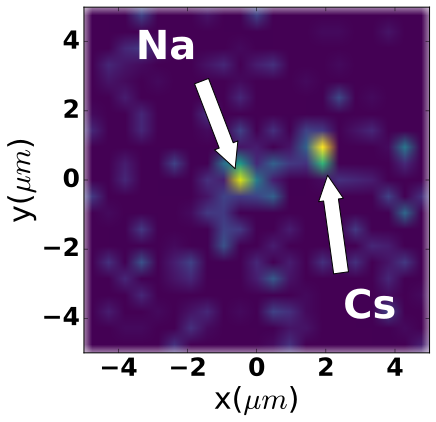
\includegraphics[width=3cm]{../../experiments/nacs_atoms/imgs/single_viridis.png}};
      }
    \end{tikzpicture}
  \end{center}
\end{frame}

\begin{frame}{Wave function size}
  \begin{center}
    \begin{tikzpicture}
      \shade[ball color=blue!90] (0, 0) circle (0.45);
      \shade[ball color=orange!90] (0.4, 0.2) circle (0.3);
      \draw[<->,line width=1] (-0.45, 0.4) -- (0.35, 0.8);
      \path (-0.05, 0.6) node[rotate=26.565,above=2pt] {$4a_0$};
      \path (0.2, -2) node[below] {\textbf{Molecule}};

      \draw[line width=1] plot[samples=200,domain=-2:2,variable=\x] ({\x + 6}, {(\x)^2 * 0.8 - 1.5});
      \draw[line width=2,orange!90!black]
      plot[samples=200,domain=-2:2,variable=\x] ({\x + 6}, {exp(-(\x)^2 * 1.3) - 0.988});
      \draw[line width=0.8] (6 - 0.8, -0.988) -- (6 + 0.8, -0.988);
      \draw[<->,line width=1] (6 - 1, 0.3) -- (6 + 1, 0.3);
      \path (6, 0.3) node[above] {$1000a_0$};
      \path (6, -2) node[below] {\textbf{Atom}};
    \end{tikzpicture}
  \end{center}
\end{frame}

\begin{frame}{Raman sideband cooling of Sodium}
  \begin{columns}
    \column{6.5cm}
    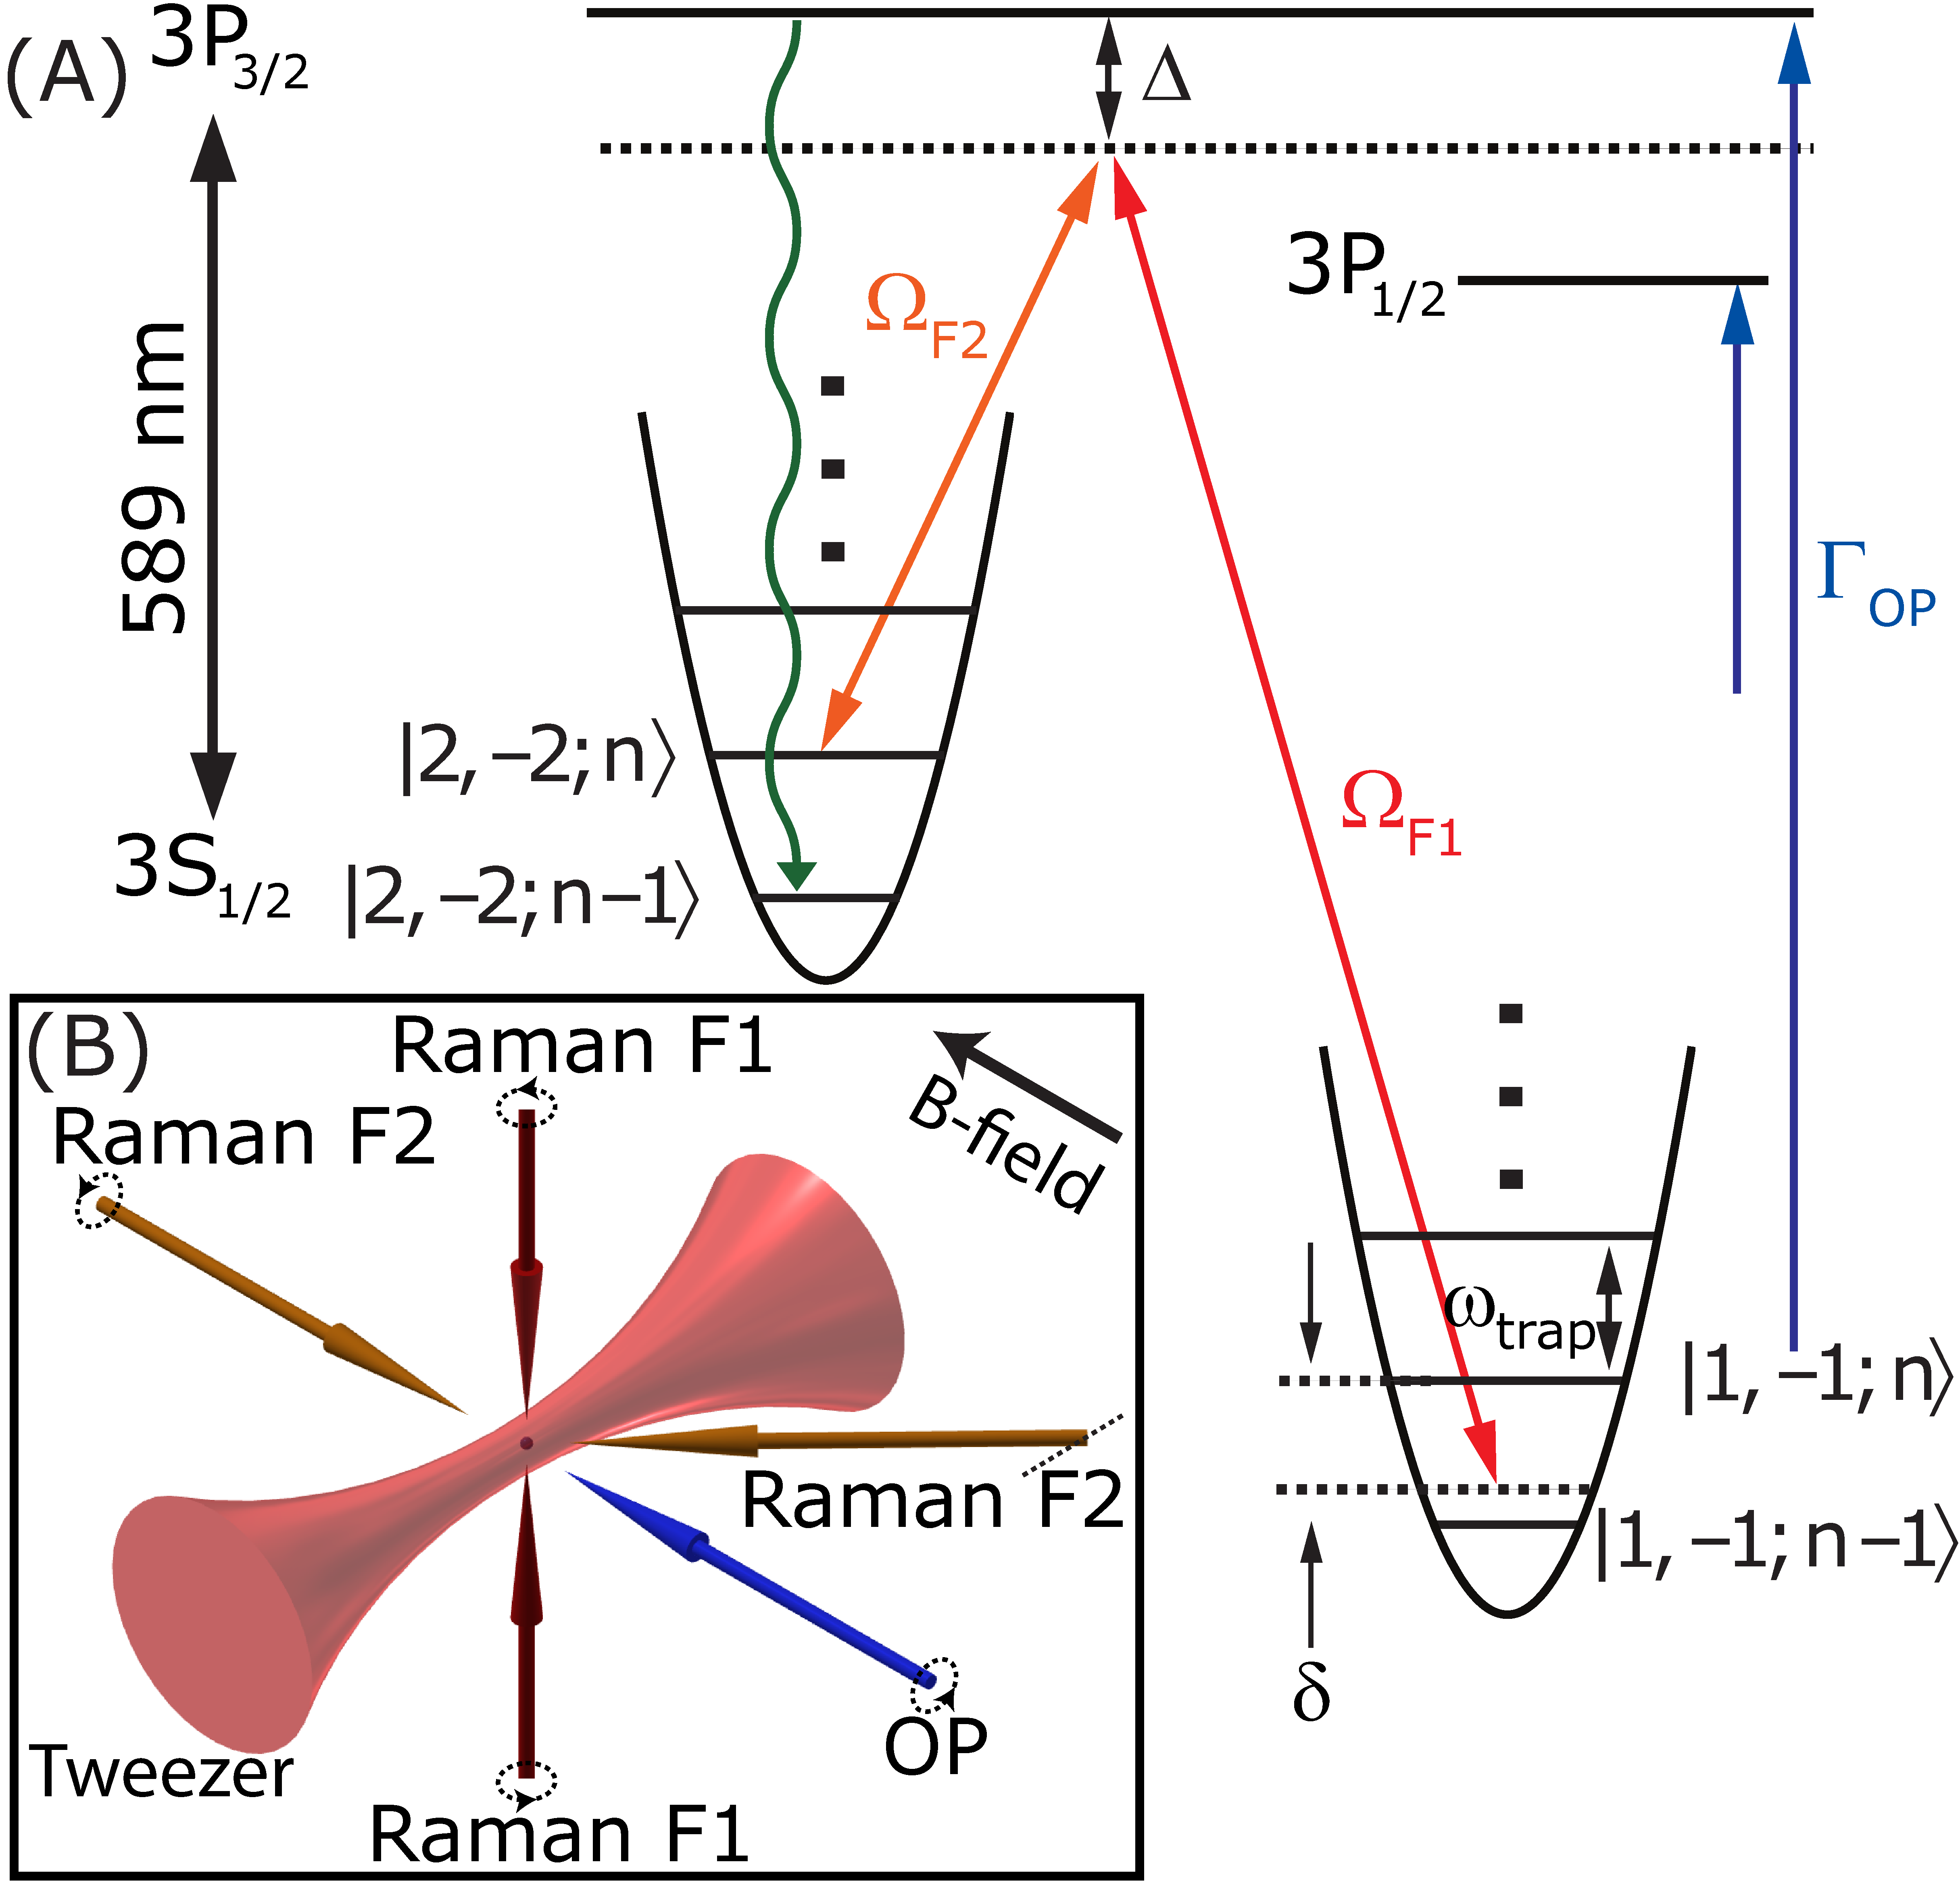
\includegraphics[width=6cm]{Na_RSC_schematic.pdf}
    \column{5cm}
    \visible<2->{
      \begin{block}{Difficulties}
        \begin{itemize}
        \item High initial temperature ($40\mu K$)
        \item<3-> High recoil heating
        \end{itemize}
      \end{block}
    }
  \end{columns}
\end{frame}

\begin{frame}{Cooling sequence}
  \tikzfading[name=fade img right,
  left color=transparent!90, right color=transparent!0]
  \begin{tikzpicture}[scale=0.75]
    % 0.0 - 1.5 axial
    % 1.5 - 2.0 OP
    % 2.0 - 3.5 axial
    % 3.5 - 4.0 OP
    % 4.0 - 5.0 radial 2
    % 5.0 - 5.5 OP
    % 5.5 - 7.0 axial
    % 7.0 - 7.5 OP
    % 7.5 - 9.0 axial
    % 9.0 - 9.5 OP
    % 9.5 - 10.5 radial 3
    % 10.5 - 11.0 OP

    %% Pulse mark
    \foreach \i in {2.0, 4.0, 5.5, 7.5, 9.5, 11.0, 13.0, 15.0, 16.5, 18.5, 20.5} {
      \draw[gray!20, line width=1.5] (\i, 1.8) -- (\i, -6.0);
    }

    %% Axial
    \foreach \i in {0, 5.5, 11.0, 16.5} {
      \fill[blue!30]
      plot[draw,samples=200,domain=\i:{\i+1.5},variable=\x] ({\x}, {sin((\x-\i) * 120)^4})
      -- cycle;
      \path (\i+1, 1) node[above,blue,align=center] {$n$-th\\order};
      \fill[blue!30]
      plot[draw,samples=200,domain={\i+2.0}:{\i+3.5},variable=\x] ({\x}, {sin((\x-\i-2.0) * 120)^4})
      -- cycle;
      \path (\i+3, 1) node[above,blue,align=center] {$(n-1)$-th\\order};
      \draw[line width=1,blue] plot[domain=\i:{\i+1.5},variable=\x]
      ({\x}, {sin((\x-\i) * 120)^4}) -- (\i+2.0, 0)
      plot[domain={\i+2.0}:{\i+3.5},variable=\x]
      ({\x}, {sin((\x-\i-2.0) * 120)^4})-- (\i+5.5, 0);
    }
    \path (0, 0.5) node[left,blue,align=center] {\textbf{Axis 1}\\\textit{Axial}};

    %% Radial 2
    \foreach \i in {0, 11.0} {
      \fill[red!30]
      plot[draw,samples=200,domain={\i+4.0}:{\i+5.0},variable=\x] ({\x}, {1.5*sin((\x-\i-4.0) * 180)^4 - 2})
      -- cycle;
      \draw[line width=1,red] (\i, -2) -- plot[domain={\i+4.0}:{\i+5.0},variable=\x]
      ({\x}, {1.5*sin((\x-\i-4.0) * 180)^4 - 2}) -- (\i+11.0, -2);
    }
    \path (0, -1.5) node[left,red,align=center] {\textbf{Axis 2}\\\textit{Radial}};

    %% Radial 3
    \foreach \i in {0, 11.0} {
      \fill[black!30]
      plot[draw,samples=200,domain={\i+9.5}:{\i+10.5},variable=\x] ({\x}, {1.5*sin((\x-\i-9.5) * 180)^4 - 4})
      -- cycle;
      \draw[line width=1,black] (\i, -4) -- plot[domain={\i+9.5}:{\i+10.5},variable=\x]
      ({\x}, {1.5*sin((\x-\i-9.5) * 180)^4 - 4}) -- (\i+11.0, -4);
    }
    \path (0, -3.5) node[left,black,align=center] {\textbf{Axis 3}\\\textit{Radial}};

    %% OP
    \foreach \i in {0, 5.5, 11.0, 16.5} {
      \filldraw[fill=orange!30,draw=orange,line width=1.5]
      (\i+1.5, -6) -- (\i+1.5, -4.5) -- (\i+2.0, -4.5) -- (\i+2.0, -6) -- cycle;
      \filldraw[fill=orange!30,draw=orange,line width=1.5]
      (\i+3.5, -6) -- (\i+3.5, -4.5) -- (\i+4.0, -4.5) -- (\i+4.0, -6) -- cycle;
      \filldraw[fill=orange!30,draw=orange,line width=1.5]
      (\i+5.0, -6) -- (\i+5.0, -4.5) -- (\i+5.5, -4.5) -- (\i+5.5, -6) -- cycle;
    }
    \path (0, -5.5) node[left,orange,align=center] {\textbf{Optical}\\\textbf{pumping}};
    \draw[line width=2,orange] (0,-6) -- (23,-6);

    %% Cycle mark
    \draw[decoration={brace,mirror,raise=3pt, amplitude=10pt},decorate,line width=2]
    (0,-6) -- node[below=15pt] {\scalebox{1.5}{One cooling cycle}} (11,-6);

    \fill[white,path fading=fade img right] (11, -7) rectangle (14.5, 2.5);
    \fill[white,path fading=fade img right] (11, -7) rectangle (14.5, 2.5);
    \fill[white] (14.5, 2.5) rectangle (23, -7);

    \draw[line width=2,orange,->] (0,-6) -- (12,-6) node[right, below] {\scalebox{2}{$t$}};
  \end{tikzpicture}
\end{frame}

\begin{frame}{Raman sidebands}
  \begin{tikzpicture}
    \visible<1-2> {
      \path (1.75, 4) node {
        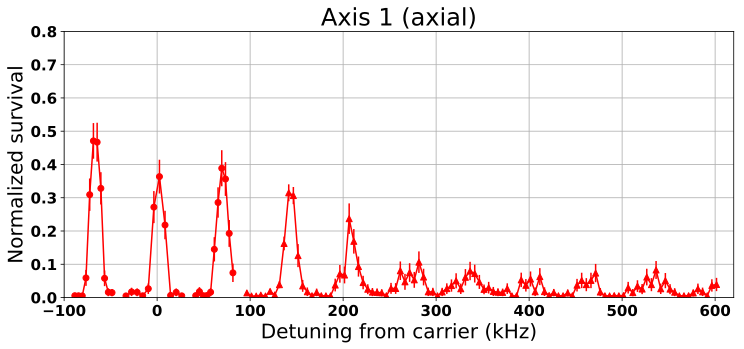
\includegraphics[width=8.5cm]{../../experiments/misc/imgs/data_spectrum_20170409_a1_before.png}
      };
      \path (0, 0) node {
        \includegraphics[width=5cm]{../../experiments/misc/imgs/data_spectrum_20170409_r2_before.png}
      };
      \path (6, 0) node {
        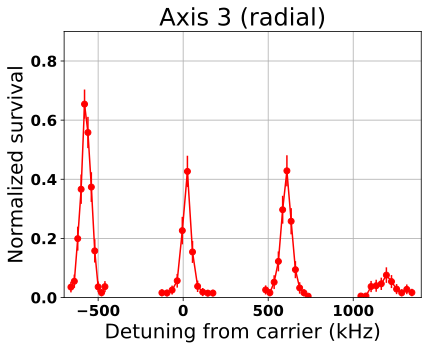
\includegraphics[width=5cm]{../../experiments/misc/imgs/data_spectrum_20170409_r3_before.png}
      };
      \visible<2> {
        \draw[red, <-, line width=1.5] (-1.4, 4.5) -- (-1.2, 5.2)
        node[above right] {1st order heating};
        \draw[<-, line width=1.5] (-0.7, 4.2) -- (-0.5, 4.8) node[above right] {Carrier};
        \draw[black!40!green, <-, line width=1.5] (0.05, 4.2) -- (0.2, 4.6)
        node[right] {1st order cooling};
        \draw[blue, <-, line width=1.5] (0.8, 3.9) -- (1.2, 4.1)
        node[right] {2nd order cooling};
        \path[magenta] (2, 3.5) node[right] {And higher orders{$\cdots$}};

        \draw[<-, line width=1.5] (-0.35, 0) -- (0, 0.8) node[right] {Carrier};

        \draw[<-, line width=1.5] (5.67, 0.1) -- (6, 0.8) node[right] {Carrier};
      }
    }
    \visible<3-> {
      \path (1.75, 4) node {
        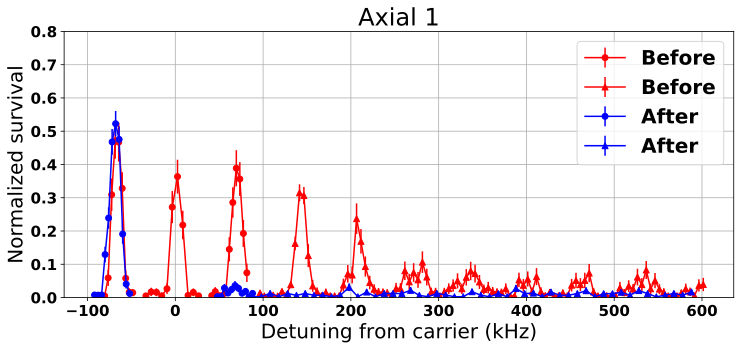
\includegraphics[width=8.5cm]{../../experiments/misc/imgs/data_spectrum_20170409_a1.png}
      };
      \path (0, 0) node {
        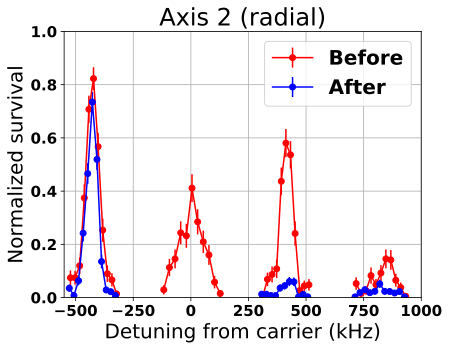
\includegraphics[width=5cm]{../../experiments/misc/imgs/data_spectrum_20170409_r2.png}
      };
      \path (6, 0) node {
        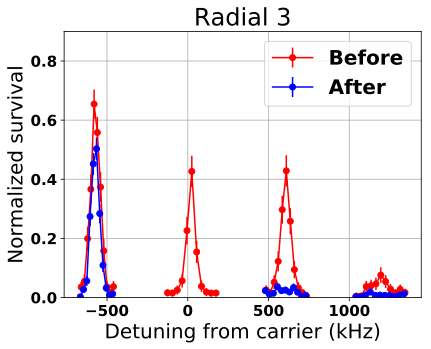
\includegraphics[width=5cm]{../../experiments/misc/imgs/data_spectrum_20170409_r3.png}
      };
    }
    \visible<4-> {
      \path[blue] (2, 4.6) node[fill=white,opacity=0.6,text opacity=1,align=center]
      {$\bm{P_{ground\ state}}$\\$\bm{93.1(2.5)\%}$};
      \path[blue] (2, 0.1) node[fill=white,opacity=0.6,text opacity=1,align=center]
      {$\bm{P_{ground\ state}}$\\$\bm{91.9(2.3)\%}$};
      \path[blue] (8, 0.1) node[fill=white,opacity=0.6,text opacity=1,align=center]
      {$\bm{P_{ground\ state}}$\\$\bm{92.9(2.5)\%}$};
      \fill[white,path fading=fade img right] (4, 2.1) rectangle (7, 6);
      \fill[white,path fading=fade img right] (4, 2.1) rectangle (7, 6);
      \fill[white,path fading=fade img right] (4, 2.1) rectangle (7, 6);
      \path (4, 4) node[fill=blue!80!white,opacity=0.8,text opacity=1,
      text=white!90!yellow,right,align=center,
      rounded corners=0.2cm,inner sep=0.2cm] {
        \textbf{3D ground state:} $79.5(3.6)\%$\\
        \textbf{Loss after cooling:} $15\%$\\\\
        \textbf{Total 3D ground state}\\
        \textbf{preparation fidelity}\\
        $67.6(3.1)\%$
      };
    }
  \end{tikzpicture}
\end{frame}

\begin{frame}{Rabi flopping (radial)}
  \begin{center}
    \visible<+->{
      \includegraphics[width=10cm]{../../experiments/rabi_flop/imgs/fit_20170409_r2_0_ba.png}\\
    }
    \visible<+->{
      Good agreement between spectrum and Rabi flopping data.
    }
  \end{center}
\end{frame}

\begin{frame}{Rabi flopping (axial)}
  \begin{center}
    \includegraphics[width=10cm]{../../experiments/rabi_flop/imgs/fit_20170409_a1_p1_ba.png}\\
    Decoherence caused by magnetic field fluctuation.
  \end{center}
\end{frame}

\begin{frame}{}
  \begin{block}{Conclusion}
    $67.6(3.1)\%$ ground state preparation fidelity {\small ($79.5(3.6)\%$ without loss)}
  \end{block}
  \vspace{1cm}
  \begin{block}{Improvements}
    \begin{itemize}
    \item Reduce off-resonance scattering from Raman beams
    \item Reduce magnetic field fluctuation
    \item Reduce loss during cooling
    \end{itemize}
  \end{block}
\end{frame}

\begin{frame}{}
\end{frame}

\begin{frame}{Axial matrix element}
  \begin{center}
    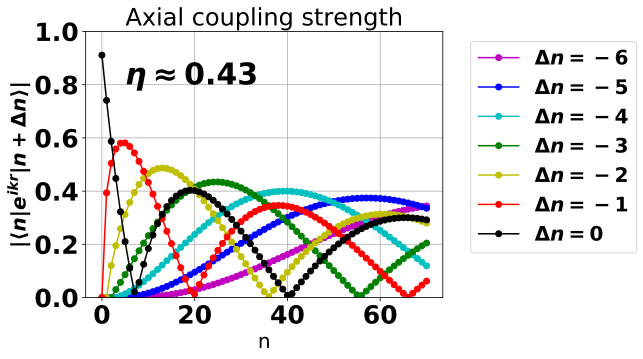
\includegraphics[width=6.5cm]{{../../calculations/sideband_strength/imgs/coupling_0.43_0-6}.png}
  \end{center}
\end{frame}

\begin{frame}{Radial 2 matrix element}
  \begin{center}
    \includegraphics[width=6.5cm]{{../../calculations/sideband_strength/imgs/coupling_0.35_0-2}.png}
  \end{center}
\end{frame}

\begin{frame}{Radial 3 matrix element}
  \begin{center}
    \includegraphics[width=6.5cm]{{../../calculations/sideband_strength/imgs/coupling_0.29_0-2}.png}
  \end{center}
\end{frame}

\end{document}
